\chapter{Realisierung}
\label{cha:realisierung}
In diesem Kapitel werden zunächst die Technologien besprochen, die für die Umsetzung nötig waren. Anschließend wird ausgeführt wie das Konzept schlussendlich umgesetzt wurde. Dabei wird auch das Design besprochen und auf Probleme bei der Umsetzung eingangen.

% Abschnitt: Technologien
\section{Technologien}
\label{sec:grundlagen:technologien}
Dieser Abschnitt dient dazu die genutzten Technologien kurz vorzustellen und eventuell auf Vor- und Nachteile sowie auf Besonderheiten einzugehen.

\subsection{Unity}
\label{subsec:realisierung:technologien:unity}
Unity ist eine Game-Engine der Firma \textit{Unity Technologies}. Die Entwicklungsumgebung der Game-Engine unterstützt mit integrierten Tools für Animation, Partikel-Systemen, Audio-Mixing und Tilemaps den gesamten Arbeitsablauf zum Erstellen von Spielen \cite{unity_mobile}. Unity erlaub dabei das Entwickln von Spielen auf die meisten Plattformen (Windows, Android, iOS, XBox, uvm.) und unterstützt dabei sowohl 2D-, als auch 3D-Spiele.

Im Folgendem werden die Vorteile, als auch die Nachteile der Spieleentwicklung mit Unity erläutert. Im Anschluss werden einige der Funktionen von Unity vorgestellt.
\subsubsection*{Vorteile}
\begin{itemize}
    \item Die von Unity verwendete Programmiersprache ist C\#, welche sehr ähnlich zu Java ist. Java als Programmiersprache ist uns (dem Team) gut geläufig, wodurch wir uns die Einarbeitungszeit in eine Programmiersprache ersparten.
    \item Unity unterstützt, die von uns vorgesehene Levelgestaltung, mit \textit{Tilemaps}. Damit wird das Bauen von Levelstrukturen und Hindernissen einfacher und schneller.
    \item Unity bietet durch seinen Asset-Store eine Großzahl an Vorlagen von jedlichen Spielfiguren, Plugins und weiteren vordefienierten Spielfunktionen (teils kostenpflichtig).
    \item Unity besitzt viele vordefinierte Funktionen, die dem Entwickler die Arbeit erheblich vereinfachen. Zum Beispiel können die im Spiel verwendete \textit{Physics} einfach konfiguriert werden und müssen nicht extra entwickelt werden.
    \item Das Builden der Anwendung auf Android (die Zielplattform) ist sehr schnell und unkompliziert. Allgemein besitzt Unity und Android eine gute Kompatibilität.
\end{itemize}

\subsubsection*{Nachteile}
\begin{itemize}
    \item Da für jedes selbst entwickelte Skript eine eigene Datei erstellt werden muss und Unity sehr viele Funktionen bereits implementiert hat, wird die Entwicklungsumgebung schnell unübersichtlich. Das erschwert das Arbeiten und verlangsamt den Arbeitsprozess.
    \item Unity ist eine (für uns) eine komlett neue Arbeitsumgebung. Die Levelgestaltung im Editor und unterschiedlichen Funktionen, die mit Unity einhergehen sind ungewohnt.
    \item Das Arbeiten im Team erfordert die Einbeziehung von Git, jedoch besitzt Unity keine gute Kompatibilität mit Git. Es treten nach dem Mergen oft Probleme auf und erschweren ein schnelles Entwickeln der Anwendung.
\end{itemize}

Unity ist eine Entwicklungsumgebung für Spiele mit geringer Einarbeitungszeit. Unity bietet mit seinen Funktionen die optimale Programmierumgebung um ein 2D-Jump 'n' Run-Muliplayer-Spiel zu erstellen. Einige der Funktionen werden im Folgenden vorgestellt.

\begin{description}
    \item[GameObjects] \hfill \\* Ein GameObject ist die Basisklasse für alle Entitäten einer Unity-Szene.
    \item[Components] \hfill \\* Eine Component ist eine Basisklasse für alles was mit GameObject verbunden ist.
    \item[Collider] \hfill \\* Collider sind in Unity dafür zuständig zu erkenn ob sich zwei Gameobjects berühren. Dadurch kann festgestellt werden ob der Spieler zum Beispiel auf der Spielfläche sich befindet oder ein Power-Up eingesammelt hat.
    \item[RayCasting] \hfill \\*
        RayCasting prüft wie ein Collider auf eine Kollision zwischen zwei Objekten. Der Vorteil ist allerdings das auch die Richtung der Kollision (oben, unten, rechts, links) bestimmt werden kann. Zudem kann man auch erkennen, wenn die Objekte kurz vor einer Kollision stehen, das ist insbesondere für den Walljump äußerst praktisch.
    \item[Tilemap] \hfill \\* Mit der Tilemap können schnell 2D-Ebenen erstellt werden. Tilemaps bestehen aus einem Gitter. Die verschiedenen Felder des Gitters können mit \textit{Tiles} gefüllt werden. Diese Tiles bilden die Spieloberfläche auf der der Spieler sich bewegen kann. Sind verschiedene Tiles verfügbar können schnell und einfach neue Level ganz einfach gezeichnet werden. \\ 
        Bei der Gestaltung von eigenen Tiles ist besonders wichtig, dass die Tiles zueinander passen, also bei einer Anordnung in einer horizontalen Reihe sollten die Tiles rechts und links ineinander übergehen.
        
        
    \item[Prefabs] \hfill \\* Werden GameObjects mehrfach benötigt und ändern sich in ihrem Verhalten und Aussehen nicht, können Prefabs verwendet werden. Anstatt eine GameObject zu duplizieren und jedes Duplikat bei einer Änderung individuell zu ändern, haben Prefabs den Vorteil die vorgenommene Änderung auf alle Prefabs dieser Art zu übernehmen.
    \item[Inspector] \hfill \\* Projekte im Unity Editor bestehen aus GameObjects die Skripte, Sounds, usw. enthalten. Der Inspector zeigt detaillierte Informationen über jedes Component des ausgewählten GameObjects und erlaubt es dem Entwickler die Daten zu verändern.
    \item[Asset Store] \hfill \\* Der Asset Store ist wie der Nameschon sagt ein Store der viele Assets anbietet, die Entwickler dabei unterstützen ein Spiel zu entwickeln.
\end{description}

% TODO Code-Snippet aus Vortrag?

\subsection{Photon}
\label{subsec:realisierung:technologien:photon}
Um Mulitplayer zu ermöglichen wird Photon verwendet. Photon verwaltet gemeinsame Sitzungen (Räume) von Spielern und ermöglicht es so, Nachrichten und Daten zwischen den verbunden Spielern plattformübergreifend in Echtzeit zu synchronisieren \cite{photon}.

Mit Photon kann man die neben den netzwerkrelevanten Daten auch die Position und Spielerinformationen unter den Spielern teilen. Dadurch können die jewiligen Endgeräte miteinander kommunizieren und ein gemeinsames Spielen ermöglichen. Dazu stellt Photon eine Vielzahl an Methoden zur Verfügung, die es dem Entwickler ermöglicht die Verbindung zwischen den Spielern aufzubauen, Räume zu erstellen und Spieldaten auszutauschen.

Eine nützliche Funktion Photons in der Spieleentwicklung sind \textit{Remote Procedure Calls} (RPC), die es ermöglichen Methoden in anderen Adressräumen aufzurufen. Dadurch können die Spieler untereinander Methoden aufrufen und direkt miteinander kommunizieren.

\subsection{Weitere Frameworks}
\label{subsec:realisierung:technologien:frameworks}
Für das An- und Abmelden von Spieleraccount wird eine \textit{Java REST Server} erstellt, der die Nutzer verwaltet. Dabei werden mit der Registrierung Nutzer erstellt und bei der Anmeldung überprüft, ob die jeweiligen Nutzer vorhanden sind und ob die eingegeben Nutzerdaten bei der Anmeldung korrekt sind. Zusätzlich übernimmt der Server die Funktion, die Level nach dem Beendigen des vorherigen Level freizuschalten. Der Server speichert somit neben den Nutzerdaten, die Levelfreigabe der jeweiligen Nutzer. Der Server verwendet dabei eine PostgresSQL-Datenbank.

\subsection{Architektur}
\label{subsec:realisierung:technologien:architektur}
% Zusammenspiel von Photon, Unity und Server
Wie Photon und der Java REST Server mit Unity kommunizieren, zeigt Abbildung \ref{fig:realisierung:technologien:architektur}. Nach dem Start der Unity-Anwendung ist der REST-Server für die Anmeldung und die Levelauswahl zuständig. Anschließend verwaltet Photon die verschiedenen Räume und das Spiel an sich.

\begin{figure}[H]
    \begin{center}
      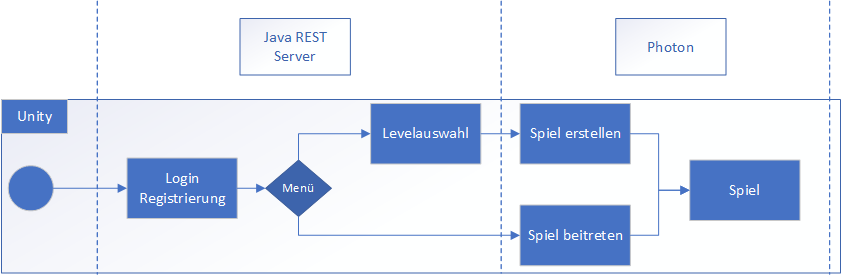
\includegraphics[width=\linewidth]{img/realisierung/Architektur}
      \caption{Architektur}
      \label{fig:realisierung:technologien:architektur}
    \end{center}
\end{figure}

%\subsection{Unity \& Mobile Applications}
%\label{subsec:implementierung:technologien:mobile}
% ich weiß nicht was da rein soll^^ TODO

\section{Umsetzung}
\label{sec:grundlagen:umsetzung}
Nachdem das Spielkonzept und die Programmierumgebung vorgestellt wurden, wird nun die Umsetzung des Spiels vorgestellt. Dabei werden wichtige Codebeispiele und die Funktionen verschiedener Spielobjekte vorgestellt. Zusätzlich wird auf das Menü, der Spielablauf und die Levelgestaltung zum Erzwingen von Teamplay eingegangen.

\subsection{Codebeispiele}
\label{subsec:implementierung:umsetzung:codebeispiele}
Um neben den verschiedenen UI-Elementen und den Leveldesigns auch die erstellte Funktionalität vorzustellen, werden kurze Codebeispiele gezeigt. Als Beispiel wird wie in Kapitel \ref{subsec:realisierung:technologien:photon} die RPC-Aufrufe kurz dargestellt und erläutert. Das Codebeispiel \ref{lst:implementierung:umsetzung:codebeispiele1} zeigt wie nach dem Start des Skripts die Methode \texttt{StartGameRPC} mit Hilfe eines RPC-Aufruf aufgerufen wird. Der Aufruf richtet sich dabei an alle Spieler, die sich in dem Raum befinden (vgl. \texttt{PhotonTargets.All}). Anschließend können weiter Parameter übergeben werden (hier der Name des zu startende Levels).

Die Methoden die über einen RPC-Aufruf erreichbar gemacht werden sollen, werden mit \texttt{PunRPC} gekennzeichnet.

\begin{lstlisting}[caption={RPC-Aufrufe}, label=lst:implementierung:umsetzung:codebeispiele1]
public class PhotonExample : PunBehaviour {

    public void Start() {        
        photonView.RPC("StartGameRPC",PhotonTargets.All,"lvl01");    
    }
    
    [PunRPC]    
    public void StartGameRPC(string sceneName) {        
        NetworkManager.Reference.StartGame(sceneName);    
    }
}
\end{lstlisting}

\subsection{Szenen und Spielobjekte}
\label{subsec:implementierung:umsetzung:realisierung}
In diesem Kapitel werden die verschiedenen Szenen und Spielobjekte vorgestellt. Dabei wird der Aufbau der Level und die Funktionsweise der Spielobjekte aufgezeigt.

\subsubsection{Menü}
\label{subsubsec:implementierung:umsetzung:realisierung:menu}

Das Menü mit dem Login und der Spielerstellung ist der Einstiegspunkt des Spiels. Der gesamte Menü-Dialog ist eine Szene, die durch aus- und einblenden von UI-Elementen das Erstellen des Spiels und das Verändern der Einstellungen ermöglicht. Der Hintergrund der Menü-Szene verwendet \textit{Parallax-Scrolling} um die ansonsten statische Spielumgebung dynamischer zu gestalten. Durch Parallax-Scrolling bewegt sich der Hintergrund stetig von rechts nach links. Zum Starten des Hauptmenüs muss der Nutzer den Usernamen und das Passwort eingeben. Er muss sich dafür registrieren und anschließend anmelden. 

Damit der Input für Nutzername und Passwort valide ist, wird überprüft, ob überhaupt etwas eingetragen wurde und ob der Input zwischen 1 und 32 Zeichen liegt. Ansonsten erscheint ein Hinweis der den Nutzer darauf hinweist.

\begin{figure}[H]
    \begin{center}
      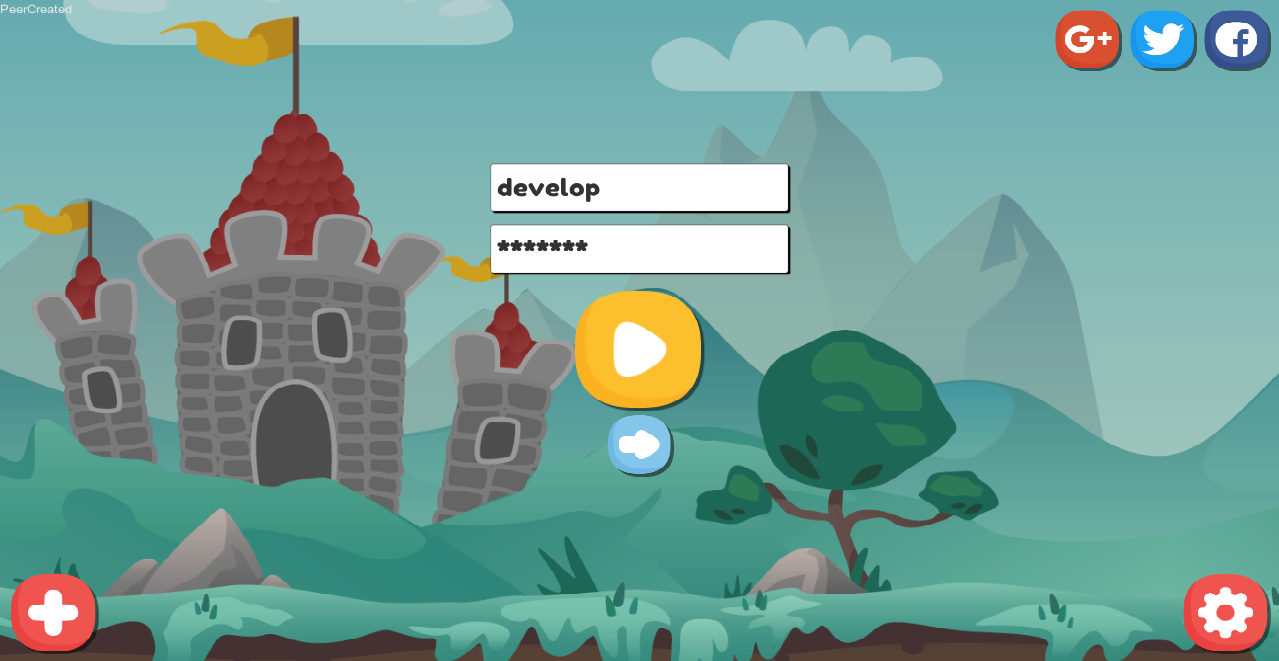
\includegraphics[width=\linewidth]{img/realisierung/Login}
      \caption{Login und Registrierung}
      \label{fig:realisierung:realisierung:login}
    \end{center}
\end{figure}

Im Hauptmenü entscheidet der Spieler, ob er ein Spiel erstellt oder einem bereits erstelltem Spiel beitritt. Zusätzlich kann der Nutzer seine Einstellungen ändern und sich Ausloggen.

\begin{figure}[H]
    \begin{center}
      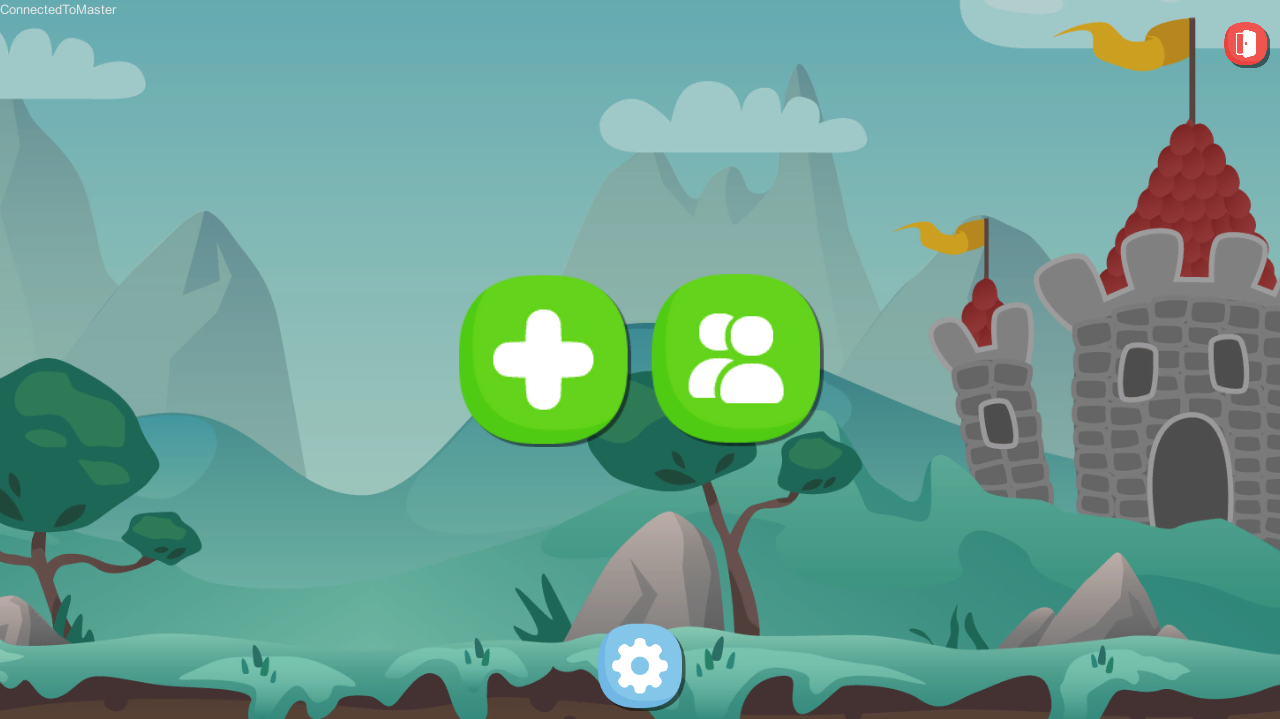
\includegraphics[width=\linewidth]{img/realisierung/menu}
      \caption{Hauptmenü}
      \label{fig:realisierung:realisierung:hauptmenu}
    \end{center}
\end{figure}

Das Spiel bietet dem Spieler die Möglichkeit die Lautstärke zu ändern. Dabei können drei verschiedene Lautstärken verändert werden. Zum einen kann die Hintergrundmusiklautstärke der jeweiligen Szene und zum anderen die In-Game-Geräsche (Springen, Schaden, Nutzen von Portalen) verändert werden. Die dritte Möglichkeit ist es das Audiofeedback nach einem Buttonklick zu variieren. Diese drei Audiomanager sind voneinander unabhängig und können so individuell verändert werden.

\begin{figure}[H]
    \begin{center}
      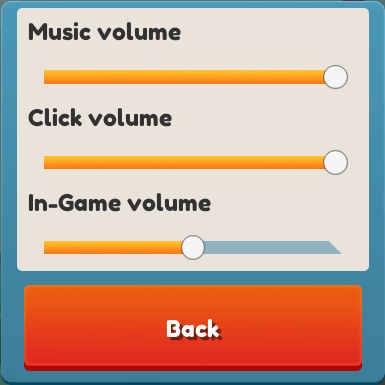
\includegraphics[width=.33\linewidth]{img/realisierung/settings}
      \caption{Lautstärkeneinstellungen}
      \label{fig:realisierung:realisierung:settings}
    \end{center}
\end{figure}

\subsubsection{Level}
\label{subsubsec:implementierung:umsetzung:realisierung:level}
Neben den Hintergrundbild sind es die Tiles, die dem jeweiligen Level das Thema verleihen. Da jedes Level sich mit einem eigenen Thema beschäftigen soll, wurden in jedem Level vier verschiedene Tiles verwendet (vgl. Abbildung \ref{fig:realisierung:realisierung:level:tiles}). Die Tiles bilden die Spieloberfläche auf der sich die Spieler bewegen können. 

\begin{figure}[H]
    \begin{center}
      
\includegraphics[width=.5\linewidth]{img/realisierung/assets/tiles_2}
      \caption{Tiles}
      \label{fig:realisierung:realisierung:level:tiles}
    \end{center}
\end{figure}

Plattformen sind wie in den meisten Jump 'n' Run-Spielen dafür zuständig die Spieler zu transportieren. Sie passen vom Thema her zu den Tiles und folgen einem vorgegebenen Pfad. 

\begin{figure}[H]
    \begin{center}
      
\includegraphics[width=.1\linewidth]{img/realisierung/assets/plattform}
      \caption{Plattform}
      \label{fig:realisierung:realisierung:level:plattform}
    \end{center}
\end{figure}

Um das Level abschließen zu können müssen die Spieler zwei Schlüssel einsammeln. Je nach Schwierigkeit des jeweiligen Levels können sie versteckt oder einfach zugänglich sein. Erst wenn beide Schlüssel (egal von welchem Spieler) eingesammelt sind, kann das Spiel beendet werden. Das Ziel des Spiels ist es eine Truhe zu erreichen. 

Damit das Level dynamischer und komplexer gestaltet wird, werden verschiedene Spielobjekte die Spieler während des Spielverlaufs unterstützen oder schaden. Im Folgenden werden diese Spielobjekte vorgestellt.

\subsubsection{Spielobjekte}
\label{subsubsec:implementierung:umsetzung:realisierung:spielobjekte}
Alle Spielobjekte haben direkten Einfluss auf das Spiel (ausgenommen die Münze). Sie können den Spielern schaden, ihr Leben erneuern oder sie transportieren. 

In Abbildung \ref{fig:keyandchest} wird der Schlüssel und die Truhe dargestellt, welche im Laufe des Spiels erreicht werden müssen, da ansonsten das Level nicht beendet werden kann. Die Spieler müssen beide Schlüssel einsammeln, damit sich die Truhe öffnet und das Level abschließt.

\begin{figure}[H]
    \centering
    \begin{subfigure}[H]{0.15\textwidth}
        
\includegraphics[width=\textwidth]{img/realisierung/assets/chest}
        \caption{Truhe}
        \label{fig:truhe}
    \end{subfigure}
    \qquad
    \begin{subfigure}[H]{0.15\textwidth}
        
\includegraphics[width=\textwidth]{img/realisierung/assets/key}
        \caption{Schlüssel}
        \label{fig:schluessel}
    \end{subfigure}
    \caption{Levelrelevante Spielobjekte}
    \label{fig:keyandchest}
\end{figure}

Das Level stellt auch Hindernisse für die Spieler. Durch bewegliche und statische Hindernisse wird das Spiel schwieriger. Abbildung \ref{fig:mace} zeig ein \textit{Mace}, dass einem vorgegebenen Pfad folgt. Statische Hindernisse in Form von \textit{Spikes} werden in Abbildung \ref{fig:spike} dargestellt. Der Spieler verliert bei Kontakt mit diesen Hindernissen Leben. Berührt er ein Hindernis zu oft oder zu lange stirbt der jeweilige Spieler und das Level muss von beiden Spielern neu gestartet werden.

\begin{figure}[H]
    \centering
    \begin{subfigure}[H]{0.15\textwidth}
        
\includegraphics[width=\textwidth]{img/realisierung/assets/mace}
        \caption{Mace}
        \label{fig:mace}
    \end{subfigure}
    \qquad
    \begin{subfigure}[H]{0.15\textwidth}
        
\includegraphics[width=\textwidth]{img/realisierung/assets/spike}
        \caption{Spike}
        \label{fig:spike}
    \end{subfigure}
    \caption{Hindernisse im Spiel}
    \label{fig:maceandspike}
\end{figure}

Sollte ein Spieler leben verloren haben, kann er durch das Einsammeln eines Power-Ups geheilt werden (vgl. Abbildung \ref{fig:eat}). Dieses Power-Up heilt ein Teil des verlorenen Lebens. 
Levelübergreifend kann der Spieler Münzen sammeln. Die Münzen haben eine kompetitive Funktion. Spieler können sich daran messen, wer eine größere Anzahl an Münzen besitzt. Eine Münze wird in Abbildung \ref{fig:coin} dargestellt.

\begin{figure}[H]
    \centering
    \begin{subfigure}[H]{0.15\textwidth}
        
\includegraphics[width=\textwidth]{img/realisierung/assets/eat}
        \caption{Power-Up}
        \label{fig:eat}
    \end{subfigure}
    \qquad
    \begin{subfigure}[H]{0.15\textwidth}
        
\includegraphics[width=\textwidth]{img/realisierung/assets/coin}
        \caption{Münze}
        \label{fig:coin}
    \end{subfigure}
    \caption{Power-Ups im Spiel}
    \label{fig:eatandcoin}
\end{figure}

Das Spielkonzept der Zusammenarbeit der Spieler wurde durch das Verwenden von Portalen und Barrieren ermöglicht. Barrieren sind nur für den Spieler durchlässig, der die selbe Farbe wie die Barriere besitzt (vgl. Abbildung \ref{fig:barriere}). Der andere Spieler kann diese Barriere nicht durchqueren. Dadurch müssen Spieler verschiedene Wege gehen oder nur ein bestimmter Spieler kann ein bestimmtes Spielobjekt (Schlüssel, Power-Up) erreichen.

Um das Spiel noch etwas dynamischer zu gestalten, können die Spieler die in Abbildung \ref{fig:portal} dargestellten Portale benutzen. Jedes Portal hängt mit einem weiteren Portal zusammen, zu dem der Spieler beim Betreten des ersten Portal teleportiert wird und umgekehrt. Dadurch können Spielbereiche erreicht werden, die der Spieler ohne das Verwenden von Portalen nicht erreichen kann.

\begin{figure}[H]
    \centering
    \begin{subfigure}[H]{0.10\textwidth}
        
\includegraphics[width=\textwidth]{img/realisierung/assets/barriere}
        \caption{Barriere}
        \label{fig:barriere}
    \end{subfigure}
    \qquad
    \begin{subfigure}[H]{0.15\textwidth}
        
\includegraphics[width=\textwidth]{img/realisierung/assets/portal}
        \caption{Portal}
        \label{fig:portal}
    \end{subfigure}
    \caption{Spielerweiternde Spielobjekte}
    \label{fig:barriereandportal}
\end{figure}

\newpage
\section{Probleme}
\label{sec:implementierung:probleme}
% Design von Assets -> Kostenlose genommen, da aufwändig
\begin{description}
    \item[Git] \hfill \\* Wie in Kapitel \ref{subsec:realisierung:technologien:unity} bereits erwähnt, ist die Kompatibilität von Unity und Git verbesserungsfähig. Bei der Entwicklung sind oft unvorhergesehene Refernzfehler aufgetreten, was das Spiel unspielbar machte und einige Zeit zum Aussbessern benötigte.
    \item[Assets] \hfill \\* Das Erstellen von UI-Elementen ist sehr aufwändig. Zusätzlich benötigt man für ein visuell ansprechendes UI-Element eine gewisse künstlerische Begabung, die nicht immer vorhanden ist. Sollen die verschiedenen UI-Elemente Animiert sein, muss jeder Frame extra gemalt werden. Diese bedeutet einen großen Aufwand mit unbefriedigenden Resultaten. Daher wurde für die Entwicklung dieser Anwendung vorgefertigte Assets verwendet.
    \item[Musik/Sounds] \hfill \\* Ähnlich wie bei den Assets sollten ursprünglich eigene Soundeffekte und Musik verwendet werden. Doch das Erstellen gestaltete sich als kompizierter und aufwändiger als gedacht. Daher haben wir auch in diesem Fall auf eine vorgefertigte und kostenlose Variante zurückgegriffen.
\end{description}





























